\documentclass[10pt]{article}

\usepackage{geometry, dsfont, tikz, float, cite}
%\usetikzlibrary{arrows,backgrounds,positioning,fit,matrix}
\usetikzlibrary{automata,arrows}

\begin{document}

\title{Tolkienizer}
\author{Sean Anderson \and Sam Payson \and Akanksha Vyas}

\section{Introduction}

The Tolkienizer is a program that uses natural language processing to create artificial
words that resemble a natural language. It uses a Hidden Markov Model to learn
trends in the language and then attempts to create words using the resulting Markov
Chain. The implementation of the project allows it to be trivially extended to
look beyond just pattens of words in a language and learn patterns 
for entire sentences.

The Tolkierizer program is free and open-source software under the GNU Public
Licence version 3. The source code is available at
\textit{https://github.com/vyasa/tolkienizer/}.

\subsection{Natural Language Processing}

Natural Language Processing (NLP) is the broad field of applying computational
analysis to natural language. It spans a huge variety of sub-fields including
morphology, parts-of-speech tagging and natural language understanding. NLP has
many important applications ranging from automatic text summarization and spam
filtering to machine translation. The Tolkienizer is similer to morphology in
that in deals with parts of words. However, instead of looking at the roots of
words, its focuses on their structure.

\subsection{Overview}
The Tolkienizer attempts to create
fake words that look and sound like they belong to a particular language. It
is named after J.R.R. Tolkien, whose artificial Elvish languages did just that
- each form of Elvish was modeled after a different Northern European language.

The Tolkienizer trains on a sample of text from a given language and learns
the patterns of how words are formed in that language. It then generates words
that it thinks are in the language, but imprecisely.
The Tolkienizer borrows from Leslie Valiant's Probably Approximately Model
(PAC) in that it needs to ensure that the model does not over-fit the learning
data\cite{val}, so that creates words that are not actually in the language, 
but seem to be. After running tests we found that The Complete Works of William
Shakespeare is too large of a training set, while the GNU English dictionary found
at \textit{/usr/share/dict/linux.words}  works well.

\section{Theoretical Background}
Hidden Markov Models (HMMs) are found to be useful in many different areas of Machine
Learning and are commonly used for NLP. HMMs are learnable probabalistic
finite state machines, considered as simple dynamic Bayesian networks
with the Markov property\cite{tech}. Before discussing them in detail I am going 
to outline the concepts of probibalistic automata, dynamic Bayesian networks and Markov Chains.

\subsection{Probibalistic Finite State Automata}
Finite state machines are models of computation characterized by
states and transitions between them. With probibalistic finite state automata, 
every transition has a probability associated with it. The transition function 
for deterministic finite state automata, given a state and a symbol, determines 
the next state for the machine. Probibalistic finite state automata have an
additional function known as the next symbol probability function, which
determines the likeliness of each transition. 

\begin{figure}[H]
\begin{center}
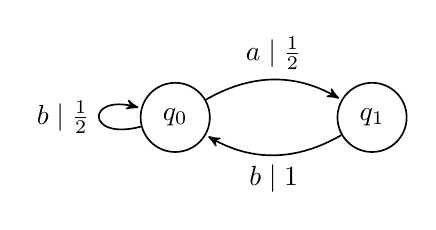
\begin{tikzpicture} [>=stealth',shorten >=1pt,node distance=2.5cm,semithick,auto]

   \node[state]                    (q0)               {$q_0$};
   \node[state]                    (q1) [right of=q0] {$q_1$};

   \path[->]    (q0) edge [bend left]   node {$a \mid \frac{1}{2}$}      (q1)
                     edge [loop left]   node {$b\mid\frac{1}{2}$}        (q0)
                (q1) edge [bend left]  node {$b\mid1$}                  (q0);
\end{tikzpicture}
\caption{A simple probibalistic finite automaton}
\label{1}
\end{center}
\end{figure}

To define it formally, a probibalistic finite state automaton is a 5-tuple
$M = ( S, \Sigma, \tau, \gamma, s_o )$ where:
\cite{bell}
\begin{itemize}
\item[] $S$ is a finite set of states.
\item[] $\Sigma$ is a finite alphabet known as the input alphabet.
\item[] $\tau: S \times \Sigma \rightarrow S$ is the transition function.
\item[] $\gamma: S \times \Sigma \rightarrow [0,1]$ is the next symbol probability
function.
\item[] $s_o \in S$ is the start state.
\end{itemize}

Finite state machines are analogous to graphs where states represent nodes and
transitions represent edges. The next subsection understands them as a
directed acyclic statistical model.

\subsection{Dynamic Bayesian Networks}
Basic probability theory addresses the issue of representing joint
probabilities as a product of conditional probabilities. However it does not 
reveal techniques for determining any dependencies between the variables in 
question. A Bayesian network is a directed acyclic graphical model for representing conditional
probabilities as well as the dependencies between the variables. A
dynamic Bayesian network represents the values of a sequence of variables at
different points in time, assuming that an event can cause another but not the
other way around \cite{vierti}. Hidden Markov Models are the canonical example
of a dynamic Bayesian network with the Markov property.

\subsection{Markov Chains}
Given a dynamic Bayesian network, the probability that the machine transitions
to a state $s_i$ depends on all the states in the path from $s_o$ to $s_{i-1}$,
where $s_o$ is the start state, as shown in equation~\ref{2}. 
\begin{equation}
\mathds{P}(s_i \mid s_{i-1}, s_{i-2}, \cdots, s_o)
\label{2}
\end{equation}

Markov chains have the beautiful property of being memoryless. The probability
that the machine will transition to a state $s_i$ depends only on state
$s_{i-1}$, as shown in equation~\ref{3}. 

\begin{equation}
\mathds{P}(s_i \mid s_{i-1})
\label{3}
\end{equation}

The Markov property holds if, for a
system, equation~\ref{3} is equivalent to equation~\ref{2}.
To define it formally, a process ia called a discrete Markov process iif 
$\forall n \geq 0$, and states $s_o, s_i, \cdots, s_i$, the following holds:\cite{dm}
\[ \mathds{P}( s_i \mid s_{i-1}, s_{i-2}, \cdots, s_o ) = \mathds{P}( s_i \mid
s_{i-1} ) \] 
\subsection{Hidden Markov Models}
Learnable probibalistic finite automata and dynamic Bayesian networks come
together to become HMMs. HMMs ask us to assume that any system under consideration, 
in our case a natural language is modeled as a Markov process. The states of
this model are hidden, but every time the model takes a transition it outputs a
measurement. Looking at this as a model of words in a natural language, the
measurement could be the next letter in the word. Given a learning set, the HMM
learns from these measurements and tries to recreate the hypothetical original
model. Figure~\ref{4} demonstrates this for two words in the English language.
\vspace{4em}
\begin{figure}[H]
\begin{minipage}[b]{0.5\linewidth}
         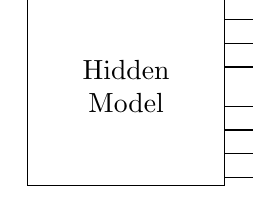
\begin{tikzpicture}
            \path[use as bounding box] (0,0) rectangle (2.5,2);
            \path[draw=black] (0,0) rectangle node[text centered,text
            width=1.5cm] {Hidden Model}(2.5,2.5);
            \path[draw=black,->] (2.5,2.4) -- node[above,blue!50] {\texttt{d}} (3.5,2.4);
            \path[draw=black,->] (2.5,2.1) -- node[above,orange!50] {\texttt{o}} (3.5,2.1);
            \path[draw=black,->] (2.5,1.8) -- node[above,purple!50] {\texttt{o}} (3.5,1.8);
            \path[draw=black,->] (2.5,1.5) -- node[above,red!50] {\texttt{m}} (3.5,1.5);

            \path[draw=black,->] (2.5,1.0) -- node[above,blue!50] {\texttt{d}} (3.5,1.0);
            \path[draw=black,->] (2.5,0.7) -- node[above,orange!50] {\texttt{o}} (3.5,0.7);
            \path[draw=black,->] (2.5,0.4) -- node[above,black!60] {\texttt{v}} (3.5,0.4);
            \path[draw=black,->] (2.5,0.1) -- node[above,purple!90] {\texttt{e}} (3.5,0.1);
         \end{tikzpicture}
         \vspace{3em}
\end{minipage}
\hspace{0.5cm}
\begin{minipage}[b]{0.5\linewidth}
         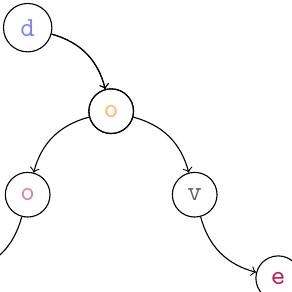
\begin{tikzpicture}[bend angle=30,node distance=1.5cm]
            \path[use as bounding box] (0,0) rectangle (3,-3);
            \path[draw=black] (0,0) node[circle,blue!50,draw=black] (d) {\texttt{d}};
            \path[draw=black] node[circle,orange!50,draw=black,below right of=d] (o1) {\texttt{o}};
            \path[draw=black] (d) edge[->,bend left] (o1);
            \path[draw=black] node[circle,purple!50,draw=black,below left of=o1] (o2) {\texttt{o}};
            \path[draw=black] (o1) edge[->,bend right] (o2);
            \path[draw=black] node[circle,red!50,draw=black,below left of=o2] (m) {\texttt{m}};
            \path[draw=black] (o2) edge[->,bend left] (m);

            \path[draw=black] node[circle,orange!50,draw=black,below right of=d] (o1) {\texttt{o}};
            \path[draw=black] (d) edge[->,bend left] (o1);

            \path[draw=black] node[circle,black!60,draw=black,below right of=o1] (v) {\texttt{v}};
            \path[draw=black] (o1) edge[->,bend left] (v);

            \path[draw=black] node[circle,purple!90,draw=black,below right of=v] (e) {\texttt{e}};
            \path[draw=black] (v) edge[->,bend right] (e);
         \end{tikzpicture}
         \vspace{3em}
\end{minipage}
\caption{A small subset of the HMM}
\label{4}
\end{figure}
\section{Implementation}
The Tolkienizer is implemented in the Go programming language, and has utf8
support so can be used for languages with character-sets that are not in
ASCII. The program has two modules: the lexer and the PFA, both of which 
are described below.
\subsection{The Lexer}
The lexer has two main components, the nReader and the demilreader.
The nReader has two levels of abstraction. As Go is a strongly
typed language, any type that implements the functions for the nReader interface
can be used for the lexer. Currently, we have code implemented for lexing
letters to make make up a word, letters to make up sequences of words and words
to make up sequences of words. Lets look at these letter/words as tokens. 
This is the first level of abstraction. At the
second level of abstraction, given any user-specified length $n$ and a reader $r$ (eg. a file)
the lexer will create a list of tokens. It can read off the reader and add the
next token to the list, creating new lists as needed. It can return the token
currently at the top of the list and also the last $n$ tokens in the list. The code
is available in \textit{lexer/nReader.go}. 

The nReader considers the end-of-word to be a space character. The delimreader,
given an abstract reader will convert all desired punctuation to a desired
character, ie. \textit{space}. This ensures that various punctuation symbols do
not confused the HMM. The PFA is responsible for creating the HMM.
\subsection{The PFA}

\section{Results}

We ran Tolkienizer on three language sets: a collection of writings in
Tolkien's Sindarin Elvish language, the GNU English dictionary, and The
Complete Works of William Shakespeare. In the case of Shakespeare, the training set
was so large that the HMM became over-trained, and never produced words that
were not in the original text. On the dictionary and Sindarin, however, we had
better results.

Sindarin created words that could very easily be mistaken for Elvish, at least
by a non-speaker. Words like ``imlain,'' ``drastannan,'' and ``maethant'' all
have a very Tolkien-esque feel, but are not in the language. The GNU English
dictionary created words that adheared to the phonetic constraints of English,
which were occasionally several ten's of characters in length.

\subsection{Example}

Here is an example using the GNU English dictionary as input:

\begin{verbatim}
$ ./tolkienizer < /usr/share/dict/linux.words
Tolkienizer v0.0
solitholacupriacetamering
spiritter
jockable
two
Coldheromebuillaboviparoo
pyrilelemembertegrous
bethness
nond
Stramadesis
Crest
Acant
burtuidness
papa
chippins
subatter
sub
brodiacarquieting
considicier
leemeiku
flags
\end{verbatim}

\section{Conclusion}

\bibliography{ai}{}
\bibliographystyle{plain}
\end{document}
